\begin{slide}
    \begin{block}{Problem}
				\noindent\begin{minipage}{0.6\textwidth}
				Given a \textcolor{red}{\textbf{red circle}}, a \textcolor{blue}{\textbf{blue circle}} and \textbf{two points}, find the length of the shortest path between the two points while staying inside the blue circle and outside the red circle.
				\end{minipage}
				\hfill
				\begin{minipage}{0.3\textwidth}\raggedleft
				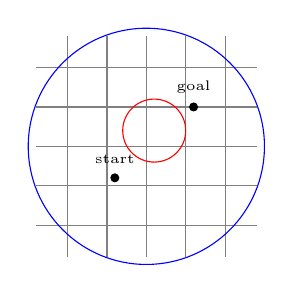
\begin{tikzpicture}[point/.style = {draw, circle,  fill = black, inner sep = 1pt}]
				\tikzstyle{help line}=[black!50]
				\draw[style=help line, step=0.5cm] (-1.4,-1.4) grid (1.4,1.4);
				\draw[color=blue] (0,0) circle (1.5cm);
				\draw[color=red] (0.1,0.2) circle (0.4cm);
				\node (start) at (-0.4, -0.4) [point, label = \tiny{start}] {};
				\node (goal) at (0.6, 0.5) [point, label = \tiny{goal}] {};
				\end{tikzpicture}
				\end{minipage}        

				\vfill
				
				Simplifications:
				\begin{itemize}
					\item Touching the circles is allowed.
					\item The direct path is always blocked by the red circle.
					\item The red circle and the two points are completely inside the blue circle.
				\end{itemize}
    \end{block}
\end{slide}

\begin{slide}
    \begin{block}{Problem}
    \begin{center}
    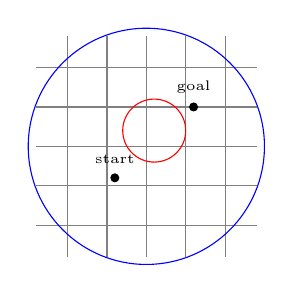
\begin{tikzpicture}[point/.style = {draw, circle,  fill = black, inner sep = 1pt}]
				\tikzstyle{help line}=[black!50]
				\draw[style=help line, step=0.5cm] (-1.4,-1.4) grid (1.4,1.4);
				\draw[color=blue] (0,0) circle (1.5cm);
				\draw[color=red] (0.1,0.2) circle (0.4cm);
				\node (start) at (-0.4, -0.4) [point, label = \tiny{start}] {};
				\node (goal) at (0.6, 0.5) [point, label = \tiny{goal}] {};
				\end{tikzpicture}
		\end{center}
		\vfill
    \end{block}
		\begin{block}{Deductions}
        \begin{itemize}
        	\item The blue circle is irrelevant.
					\item No need two check if the direct connection is possible.
        \end{itemize}
    \end{block}
\end{slide}

\begin{slide}
    \begin{block}{Problem}
			\begin{center}
				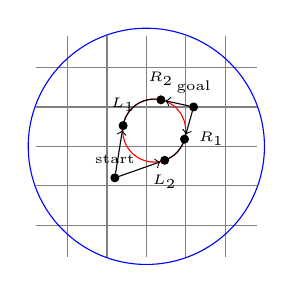
\begin{tikzpicture}[point/.style = {draw, circle,  fill = black, inner sep = 1pt}]				
				\tikzstyle{help line}=[black!50]
				\draw[style=help line, step=0.5cm] (-1.4,-1.4) grid (1.4,1.4);
				\draw[color=blue] (0,0) circle (1.5cm);
				\draw[color=red] (0.1,0.2) circle (0.4cm);
				\node (start) at (-0.4, -0.4) [point, label = \tiny{start}] {};
				\node (goal) at (0.6, 0.5) [point, label = \tiny{goal}] {};
				\node (L1) at (-0.295077, 0.262564) [point, label = \tiny{$L_1$}] {};
				\node (L2) at (0.232782,  -0.177318) [point, label = below:\tiny{$L_2$}] {};
				\node (R1) at (0.485034, 0.0916094) [point, label = right:\tiny{$R_1$}] {};
				\node (R2) at (0.185554,  0.590744) [point, label = \tiny{$R_2$}] {};
				\draw[->] (start) -- (L1);
				\draw[->] (start) -- (L2);
				\draw[->] (goal) -- (R1);
				\draw[->] (goal) -- (R2);
				\draw (0.1, 0.2) ++( 171.001:.4) arc ( 171.001:77.6499:.4);
				\draw (0.1, 0.2) ++(-70.6126:.4) arc (-70.6126:-15.7224:.4);
				\end{tikzpicture}
				\end{center}

    \end{block}
    \begin{block}{Solution}
        \begin{itemize}
        	\item Compute \textbf{tangents} of the red circle going through start and end.
        	\item Compute the length of \textbf{circle segments} between the touching points $L_{1,2}, R_{1,2}$.
        	\item Find the minimum length of the four paths $start \rightarrow L_{1,2} \rightarrow R_{1,2} \rightarrow end$.
        \end{itemize}
    \end{block}
\end{slide}
